
\section{Mediciones}

\subsection{Medicion de $f_o$}

Para la medicion de la frecuencia de resonancia, se conecta el circuito a tope. El esquema es el siguiente:

\begin{figure}[h]
    \centering
    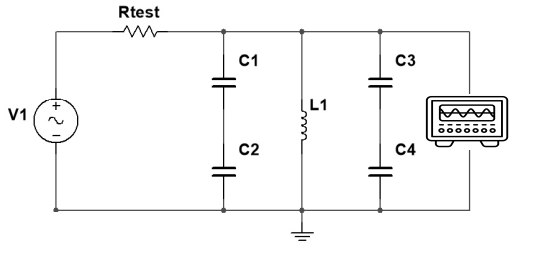
\includegraphics[width=0.5\textwidth]{Imagenes/medicion_fo.png}
    \caption{Medicion de $f_o$}
    \label{fig: de la frecuencia de resonancia $f_o$}
\end{figure}

La resistencia Rtest tiene que ser del orden de $R_p$, por lo tanto inicialmente se utilizo una resistencia de 1k$\Omega$. Una vez realizada la conexion, se varia la frecuencia 
del generador de señales de menor a mayor hasta encontrar la frecuencia de resonancia. Tenemos que considerar que el osciloscopio tiene una capacidad de entrada, por lo tanto 
esta capacidad paracita puede afectar la medicion de la frecuencia de resonancia. 


La medicion $f_o1$:

\begin{equation}
    f_o1 = 12 MHz 
\end{equation}


A continuacion mediremos la frecuencia de resonancia $f_(o2)$, para esto se utilizara una resistencia de 1k$\Omega$ y ademas, se agrega el capacitor $C_F$ en paralelo al inductor y los capacitores.
El esquema es el siguiente:

\begin{figure}[h]
    \centering
    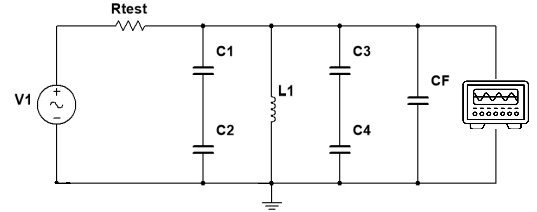
\includegraphics[width=0.5\textwidth]{Imagenes/medicion_fo2.png}
    \caption{Medicion de $f_o2$}
    \label{fig: de la frecuencia de resonancia $f_(o2)$}
\end{figure}

La medicion $f_o2$:

\begin{equation}
    f_o2 = 10.5 MHz
\end{equation}

Para obtener la frecuencia de resonancia $f_o$ se debe obtener $C_o$ apartir de estas ecuaciones:

\begin{equation}
    f_o1 = \frac{1}{2\pi\sqrt{L(C_T + C_o)}}
\end{equation}

\begin{equation}
    f_o2 = \frac{1}{2\pi\sqrt{L(C_T + C_o + C_F)}}
\end{equation}

Donde $C_T$ es igual 177 pF. Despejando $C_o$ de estas ecuaciones obtenemos:

\begin{equation}
    (\frac{f_o1}{f_o2})^2 = \frac{C_T + C_o + C_F}{C_T + C_o}
\end{equation}

\begin{equation}
    C_o = \frac{C_T \cdot (f_o2^2 - f_o1^2) + C_F f_o2^2}{f_o1^2 - f_o2^2}
\end{equation}

El capacitor $C_F$ es de 100pF y $C_o$ es de:

\begin{equation}
    C_o = 149,7 pF
\end{equation}

Con este valor damos cuenta que la capacidad agregada del osciloscopio es comparable al del circuito, por lo tanto modificara la medicion afecta el resultado.
Ahora determinaremos el valor de la inductancia $L$:

\begin{equation}
    L = \frac{1}{(2\pi f_o1)^2} \cdot \frac{1}{C_T + C_o} = 0.54 \mu H
\end{equation}

Con este valor determinamos el valor de la frecuencia de resonancia $f_o$:

\begin{equation}
    f_o = \frac{1}{2\pi\sqrt{L \cdot C_T}} = 16.27 MHz
\end{equation}

\subsection{Medicion de $BW$}

Para la medicion del ancho de banda, se utiliza el esquema de la figura \ref{fig: de la medicion del ancho de banda}:

% Colocar imagen abajo del texto de arriba
\begin{figure}[h]
    \centering
    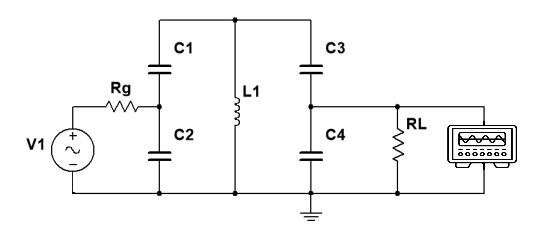
\includegraphics[width=0.5\textwidth]{Imagenes/medicion_bw.png}
    \caption{Medicion de $BW$}
    \label{fig: de la medicion del ancho de banda}
\end{figure}

La medicion del ancho de banda variaremos la frecuencia hasta encontrar el pico maximo de amplitud en la salida. Las mediciones son las siguientes:

% tabla con 3 columnas y 4 filas, frecuencia de corte inferior central y corte superior. Amplitud y frecuencia
\begin{table}[h]
    \centering
    \begin{tabular}{|c|c|c|}
    \hline
    \rowcolor[HTML]{C0C0C0} 
    \textbf{Medicion} & \textbf{Amplitud} & \textbf{Ancho de banda} \\ \hline
    Frecuencia de corte inferior            & 2.87 V             & 12.2 MHz                \\ \hline
    Frecuencia central         & 4.06 V             & 12.6 MHz                \\ \hline
    Frecuencia de corte superior            & 2.87 V             & 13 MHz                \\ \hline
    \end{tabular}
\end{table}

El ancho de banda es:

\begin{equation}
    BW = 13 - 12.2 = 0.8 MHz
\end{equation}

\subsection{Medicion de $R_p$}

Para la medicion de la resistencia de perdida, se utiliza el esquema de la figura \ref{fig: de la medicion de la resistencia de perdida}:

\begin{figure}[h]
    \centering
    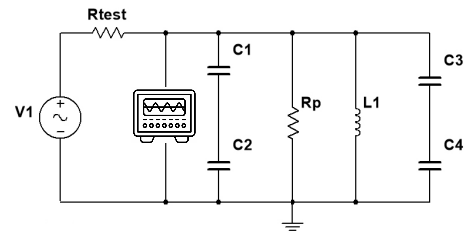
\includegraphics[width=0.8\textwidth]{Imagenes/medicion_rp.png}
    \caption{Medicion de $R_p$}
    \label{fig: de la medicion de la resistencia de perdida}
\end{figure}

Tenemos que colocar la frecuencia del generador de onda en la frecuencia de resonancia $f_o$, ya que la reactancia inductiva y capacitiva se anulan.
Por lo tanto nos quedara la resistencia de test $R_{test} = 1k\Omega$ en serie con la resistencia de perdida $R_p$. Por lo tanto realizando el divisor resistivo:

\begin{equation}
    V_{osciloscopio} = V_{B1} \cdot \frac{R_p}{R_p + R_{test}}
\end{equation}

Y despejando $R_p$ obtenemos:

\begin{equation}
    R_p = \frac{R_{test} \cdot V_{osciloscopio}}{V_{B1} - V_{osciloscopio}}
\end{equation}

Las mediciones son las siguientes:
% Hacer itemize con las mediciones
\begin{itemize}
    \item $V_{osciloscopio} = 2 V$
    \item $V_{B1} = 1.86 V$
    \item $R_p = 13.3 k\Omega$
\end{itemize}


\subsection{Medicion de $Z_{in}$}

Para la medicion de la impedancia de entrada, se utiliza el esquema de la figura \ref{fig: de la medicion de la impedancia de entrada}:

\begin{figure}[h]
    \centering
    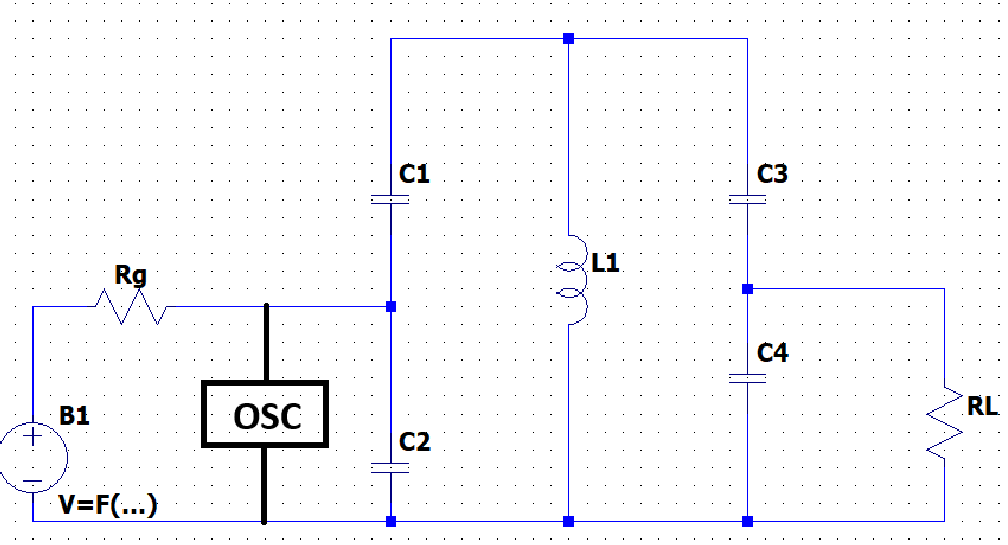
\includegraphics[width=0.8\textwidth]{Imagenes/medicion_zin.png}
    \caption{Medicion de $Z_{in}$}
    \label{fig: de la medicion de la impedancia de entrada}
\end{figure}



\subsection{Medicion de $Z_{out}$}

Para la medicion de la impedancia de salida, se utiliza el esquema de la figura \ref{fig: de la medicion de la impedancia de salida}:

\begin{figure}[h]
    \centering
    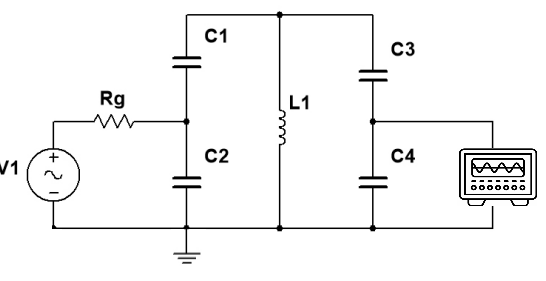
\includegraphics[width=0.8\textwidth]{Imagenes/medicion_zout1.png}
    \caption{Medicion de $Z_{out}$}
    \label{fig: Primer esquema de la medicion de la impedancia de salida}
\end{figure}

\begin{figure}[h]
    \centering
    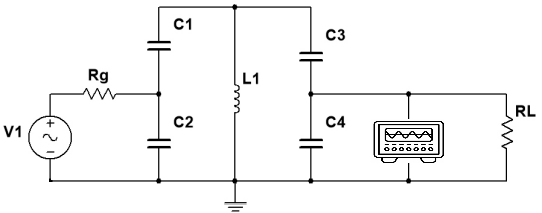
\includegraphics[width=0.8\textwidth]{Imagenes/medicion_zout2.png}
    \caption{Medicion de $Z_{out}$}
    \label{fig: Segundo esquema de la medicion de la impedancia de salida}
\end{figure}